\hfill \break
\justifying
La solución que se propone en este trabajo consiste en un prototipo \textit{wearable} sensor, que utiliza el SoC micro:bit y el sensor acelerómetro integrado para el muestreo de los patrones de movimientos realizados por el usuario, con el objetivo de realizar su clasificación mediante un sistema embebido que permita identificar la clase textual del patrón, usando en conjunto el algoritmo DTW y un modelo de Inteligencia Artificial. A partir de esta clasificación, se realiza la conformación de palabras y frases en texto, que finalmente son reproducibles sonoramente en una tarjeta de sonido cuando se hace uso de los servicios que ofrecen el proyecto \textit{TTS de Mozilla} en la red local, o los servicios especializados de \textit{Text-to-speech} ofrecidos por las nubes de compañías privadas.

\hfill \break
\justifying
Desglose de los productos particulares requeridos para cumplir la descripción de solución previa:
\begin{enumerate}
	\item Como primer propuesta al sistema embebido y prototipo mencionado, se muestra el diagrama de la solución en la Figura \ref{Diagrama}
	
	\item Código motriz como conjunto de patrones de movimiento, que en el contexto de la solución, tienen respectivamente una clasificación en una clase textual utilizada para la conformación de palabras y frases.
	
	\item El prototipo \textit{wearable} tipo guante, se compone de un par de elementos hardware escencialmente:
		\begin{itemize}
			\item El SoC micro:bit como elemento sensor principal, que implementa un IMU integrado y del cuál principalmente se utiliza el sensor acelerómetro para el muestreo de los patrones motrices.
			\item Un sensor de pulso, que a través de un gesto que puede interpretar el sensor como un pico en el ritmo cardiaco, permita al usuario indicar el inicio del muestreo de un patrón motriz y el fin de este
		\end{itemize}
		El prototipo \textit{weareable} al convertirse en el componente con el que ocurrirá la mayor parte de la interacción del usuario, funge como la interfaz principal de la solución, ofreciendo posibilidades para la configuraciones de unos pocos parámetros con el uso de los botones integrados en el SoC, y la visualización de resultados de acciones mediante animaciones en su arreglo de LEDs.
	
	\item El sistema embebido permitirá la comunicación entre el prototipo sensor, la clasificación de los patrones y la consulta de los servicios de \textit{Text-to-Speech}. Su conformación en la primer propuesta de solución considera al menos los siguientes componentes:
	\begin{itemize}
		\item Prototipo sensor \textit{wearable}
		\item Mini PC Raspberry Pi 4
		\item Tarjeta de Sonido WM8960 de Waveshare
	\end{itemize}
	
	\item La identificación de los patrones de movimiento a sus respectivas clases textuales, se podrá lograr implementando de bilbliotecas especializadas, el algoritmo DTW y un modelo de Inteligencia Artificial, que usados en conjunto permitan la clasificación eficiente de los patrones.
	
	\item La configuración de los servicios de \textit{Text-to-Speech} en red local con el proyecto \textit{TTS de Mozilla}, y el servicio especializado en la nube, permitirá el uso de al menos 2 voces femeninas y 2 voces masculinas en diferentes rangos de tono de voz y edad, al afinarse la combinación de los valores de los parámetros modificables en estos servicios.
	
	\item Artículo de publicación con el desarrollo de la solución propuesta
\end{enumerate}

\begin{figure}[!h]
	\centering
	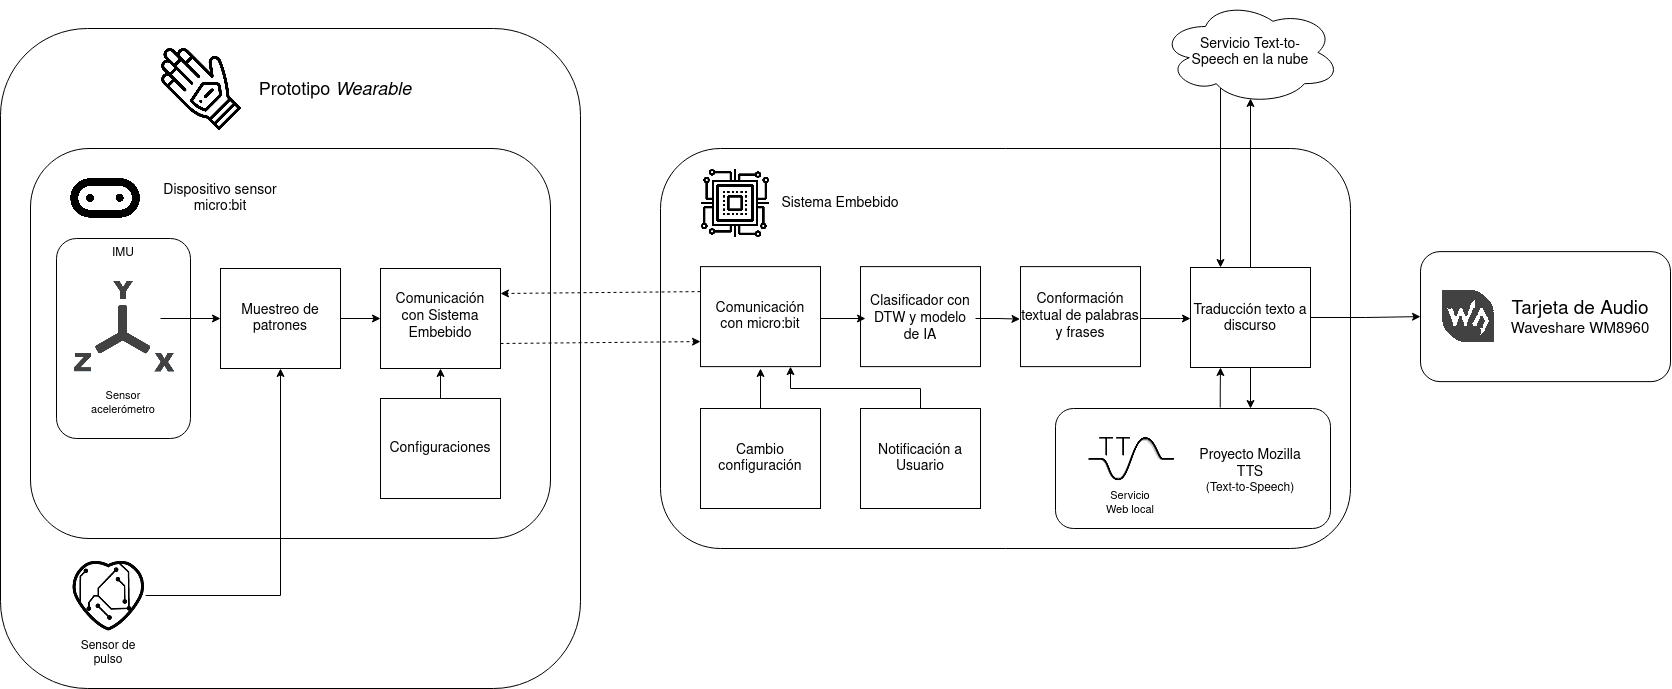
\includegraphics[width=16cm]{Imagenes/Diagrama.png}
	\caption{Diagrama como primer propuesta de solución}
	\label{Diagrama}
\end{figure}